\subsection{Relatives Vorkommen (Referenz)
}
Ein einfacher Ansatz, der als Referenz zum Finden relevanter Wörter eines Tages dient ist der, das Auftreten jedes Tokens im Tageskorpus mit dem Auftreten im Referenzkorpus ins Verhältnis zu setzen.\\
Hierbei werden um eine Vergleichbarkeit zwischen verschiednen Tagen zu gew\"ahrleisten die Frequenzen der W\"orter \"uber die Anzahl aller Tokens im Tages bzw. Referenzkorpus normiert.\\

	\emph{Formel: } 
	\begin{equation}
	sig_{freqratio}(w) = \frac{\frac{k_{day}}{n_{day}}}{\frac{k_{2014}}{n_{2014}}}
	\end{equation}
	$k_{day}$: Frequenz des Tokens an einem Tag\\
	$n_{day}$: Summe der Frequenzen aller Tokens eines Tages\\
	$k_{2014}$: Frequenz des Tokens im Referenz Zeitrahmen (2014)\\
	$n_{day}$: Summe der Frequenzen aller Tokens im Referenzzeitraum (2014)\\
	

In Abbildung \ref{pic.rel_freq} stellt die schwarze Gerade dar, wie sich der Wert der relativen Frequenz verh\"alt, wenn die Anzahl des Auftretens eines Tokens variiert. Die senkrechte roten Linien markiert die Anzahl der Tokens, bei denen das relative Auftreten dem relativen Auftreten im Referenzkorpus entspricht. Der Wert der relativen Frequenz steigt also linear bei der Steigerung der Anzahl der Tokens eines Wortes.Dies f\"uhrt zu der Problematik der \"Ubersch\"atzung von niederfrequenten W\"orter im Referenzkorpus selbst bei relativ seltenem Auftreten im Tageskorpus. Bei niederfrequenten W\"ortern ist der Anstieg der Gerade sehr viel steiler.\\
Um diesem Problem gerecht zu werden hilft es ein Ma\ss f\"ur die Relevanz eines Wortes finden, welches ein geringe \"Uberschreitung des relativen Anteils im Referenzkorpus weniger goutiert als eine h\"ohere. Der Ansatz des Poisson Ma\ss es (\ref{subsec.poisson}) versucht dem gerecht zu werden.\\
\begin{figure}[h!]
    \centering
    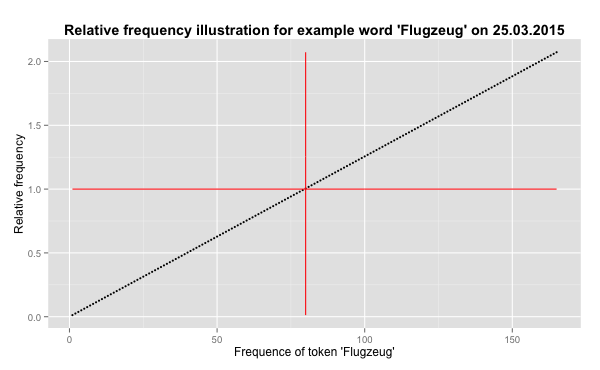
\includegraphics[width=1\textwidth]{pictures/relfreqFlugzeug.png}
    \caption{Illustration der relativen Frequenz des Tokens \enquote{Flugzeug} am 25.03.2015}\label{pic.rel_freq}
\end{figure}



\subsection{Poisson-Maß}\label{subsec.poisson}
Die Idee dieses Ansatzes ist es ein Maß zu nutzen, das die Wahrscheinlich Ausdrückt die gemessene Anzahl von Tokens eines Wortes an einem Tag zu beobachten. Auch hier wird zur Erstellung des Maßes  das Referenz

korpus des letzten Jahres genutzt. Die Annahme dieses Ansatzes ist nun, dass dieser Wahrscheinlichkeit die Poisson-Verteilung zugrundeliegt.\\
Die Formel \ref{equ.poisson} ist die Poisson-Verteilung nach \cite[S. 338 ff]{heyer06}.
	\begin{equation}\label{equ.poisson}
	P_\lambda(k) = \frac{\lambda^{k}}{k!}  \cdot e^{-\lambda}
	\end{equation}
	$\lambda$: Welche Frequenz wird erwartet \\
	(relativer Anteil im Referenzkorpus $\cdot$ Umfang des Tageskorpus)\\
	$k$: tats\"achliches Auftreten von einem Wort k\\
	$P_\lambda(k)$: Erwartete Wahrscheinlichkeit meine Beobachtung k


In Abbildung \ref{pic.poisson_algemein} ist exemplarisch die Wahrscheinlichkeit der Beobachtung der Token-H\"aufigkeit des Wortes Flugzeug abgebildet. Die Annahme besagt nun, dass je kleiner die Wahrscheinlichkeit
ist, desto relevanter erscheint ein Wort. \\

\begin{figure}[h!]
    \centering
    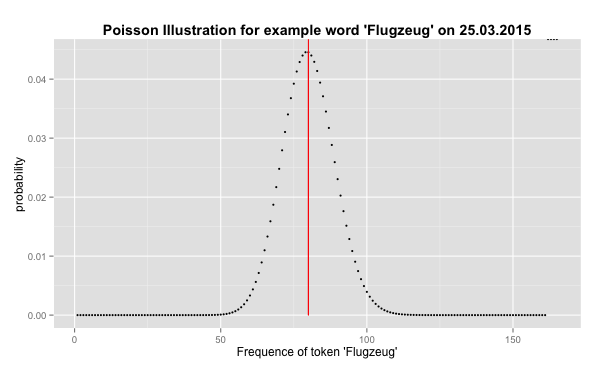
\includegraphics[width=1\textwidth]{pictures/poissonVerteilungFlugzeug.png}
    \caption{Illustration der Poissonverteilung des Token \enquote{Flugzeug} am 25.03.2015}\label{pic.poisson_algemein}
\end{figure}

An der Darstellung wird ein Nachteil dieser Methode deutlich. Nicht nur, wenn ein Token unerwartet oft beobachtet werden kann, auch wenn er seltener als erwartet beobachtet werden kann sinkt die Wahrscheinlichkeit nach diesem Modell beobachtet zu werden und es erscheint als relevantes Wort. Dieses Problem \"ost die im Folgenden beschriebene Transformation.\\

Ein weiteres Problem stellt der Rechenaufwand f\"ur diese Methode dar, da die Fakult\"at des tats\"achlichen Auftretens $k$ eines Wortes berechnet werden muss. Die Herrleitung eines einfacher zu berechnenden 
equivalenten Ma\ss es liefert \cite[S. 338 ff]{heyer06}. Zu erw\"ahnen ist, dass im Kontext dieser Herleitung wird das Ma\ss allerdings nicht zur Bestimmung von in dieser Arbeit als relevant angesehenen Einzelw\"ortern genutzt. Sondern zur Bestimmung von signifikanten Kookurenzen. \\
Die Hergeleitete Formel \ref{equ.poisson_mass} liefert drei Vorteile. Eine Berechnung der Fakult\"at ist nicht notwendig, die Anwendung des Logarithmus liefert ein positiven Wert f\"ur unwahrscheinliche Beobachtungen, wobei die differenzen gereade bei unwahrscheinlichen Beobachtungen st\"arker ins Gewicht fallen und yu letzt werden die Wahrschinlichkeiten f\"ur seltener als erwartete Tokenzahlen nicht ber\"ucksichtigt. 
 \begin{equation}\label{equ.poisson_mass}
		sig_{poisson}(w) = \frac{k(\log(k)-\log(n\cdot p) -1 ))}{\log(n)} 
 \end{equation}
 k:= Anzahl der Token von w in Tagesbericht\\
n := Anzahl der Tokens in Tagesbericht\\
p := relativer Anteil eines Tokens am Jahreskorpus\\

Die Abbildung \ref{pic.poisson_mass} illustriert die Entwicklung des Poissonma\ss es bezogen auf die Variation des Vorkommens des Tokens Flugzeug. Hier wird sichtbar, dass die unterrepr\"asentetion keinen positiven Wert erzeugt und somit keinen Einfluss auf eine nach diesem Ma\ss  geordnete Liste hat. In der Praxis sind gen\"ugend positive Werte dieses Ma\ss es zu beobachten.\\
Die Formel \ref{equ.poisson_mass} wurde im praktischen Teil dieser Arbeit genutzt.\\
\\ \\Todo: Wort satz anzahl erwaehnen \\ \\ 

% Hier Beispiel Flugzeug
\begin{figure}[h!]
    \centering
    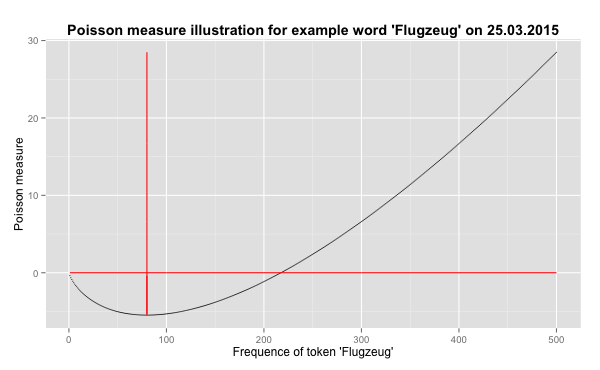
\includegraphics[width=1\textwidth]{pictures/poissonMeasureFlugzeug.png}
    \caption{Illustration des Poisson Ma\ss es des Tokens \enquote{Flugzeug} am 25.03.2015}\label{pic.poisson_mass}
\end{figure}


  
\begin{frame}{Einschub – Wortzahl vs. Satzzahl}
	\begin{itemize}
		\item{Bei der Referenz wird mit Satzzahlen gearbeitet}
		
		\item{Jeder Satz hat im Schnitt gleiche Anzahl von W\"ortern ($\approx 10$)\\
			\begin{equation}
				\frac{Satz_{heute}}{Satz_{jahr}} \approx \frac{Token_{heute}}{Token_{Jahr}}
			\end{equation}
			}
		\item{Zur \"Uberpr\"ufung sp\"ater mehr}
	\end{itemize}
\end{frame}


 
\subsection{Termfrequenz inverse Dokumentenfrequenz (tf-idf)}
 \begin{equation}
sig_{tf idf}(w) = \frac{k}{\max(K)} \cdot \log ( \frac{365}{|documentdays(w)|})
\end{equation}

\subsection{Termfrequenz inverse Dokumentenfrequenz inverse Quellenfrequenz (tf-idf-isf)}
\emph{Idee: } W\"orter sind dann interessant, wenn sie an einem Tag in m;glichst vielen verschiedenen Quellen gennant werden.\\
Als Quelle definieren wir die Serveradresse einer Quelle. Diese wird mittels eines regul\"aren Ausdrucks aus den zugeordneten Quellen in der MySQL-Datenbank ermittelt. Als Gesamtzahl der Quellen verwenden wir alle an einem Tag den W\"ortern zugeordnete Quellen.\\
Das entstandene Signifikanzma\ss wird wie folgt definiert:
 \begin{equation}
sig_{tf idf isf}(w) = sig_{tf idf}(w) \cdot \log ( \frac{Q_d}{q_d(w)})
\end{equation}
Analog zur inversen Dokumentenfrequenz wird also das tf-idf-Signifikanzma\ss  mit dem Logarithmus der inversen relativen Anzahl der Quellenfrequenz multipliziert. $Q_d$ ist die Anzahl aller erw\"ahnten Quellen an einem Tag $d$ und $q_d()$ bildet ein Wort auf die Anzahl der Quellen ab, in denen das Wort an Tag $d$  erw\"ahnt wird. 
